\section{Anwendung der Differential- und Integralrechnung}

\subsection{Orthogonale Trajektorien}
\begin{tabular}{ll}
\parbox{4.5cm}{
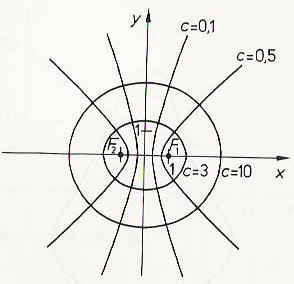
\includegraphics[height=4cm]{./bilder/orthoTrajekt.png}
}
& 
\parbox{14.5cm}{
Die orthogonalen Trajektorien schneiden alle Kurven der gegebenen Kurvenschar
$y=f(x,c)$ im rechten Winkel (orthogonal).\\
\textbf{Vorgehen:} \\
1. Kurvenschar $y=f(x,c)$ nach $c$ auflösen\\
2. $c$ in der abgeleiteten Gleichung ersetzen\\
3. $y'$ durch $-\frac{1}{y'}$ ersetzen\\
4. DGL auflösen (sofern nötig...)
}
\end{tabular}
\newline
\vspace{0.50cm}\\
Beispiel:\\
Gesucht: Orthogonalen Trajektorien der Kurvenschar $y=c \cdot x$ mit $c \in \mathbb{R}.$\\
Die Differentialgleichung ergibt sich mit $c=y'$ zu $y=y' \cdot c.$\\
Für die orthogonalen Trajektorien gilt also: $y=-\frac{1}{y'}*x.$\\
Diese Gleichung kann zu $y \cdot y'=-x$ umgeformt werden.\\
Durch Integration folgt: $\frac{1}{2} y^{2}=-\frac{1}{2} x^{2}+c_{1}$, also $x^{2}+y^{2}=k$\\
Das sind für $k>0$ konzentrische Kreise um den Nullpunkt.\\
\newline
Info: Die Kreise sind Orthogonaltrajektorien der Hyperbeln und umgekehrt.\\
$\frac{r^{\prime}}{r}=f(\varphi, r) \quad \stackrel{\text {orthogonal }}{\xrightarrow{\hspace{1.5cm}}} \quad \frac{r^{\prime}}{r}=-\frac{1}{f(\varphi, r)}$\\